%! TEX root = 'main.tex'

\section{Background}
\label{sec:ktoctou-background}


%TOCTOU is a vulnerability class caused by changes in a system between checking a condition and using that check results. Typically, a variable or system state changes after it passes the sanity check. It is a classic vulnerability, mostly amount file system APIs. Many previous research works have addressed it~\cite{dean2004fixing}~\cite{borisov2005fixing}. Before introducing the relatively new kernel-level TOCTOU, we first briefly describe the classic TOCTOU as shown in~\autoref{fig:toctou}.

%\begin{figure}[th]
%	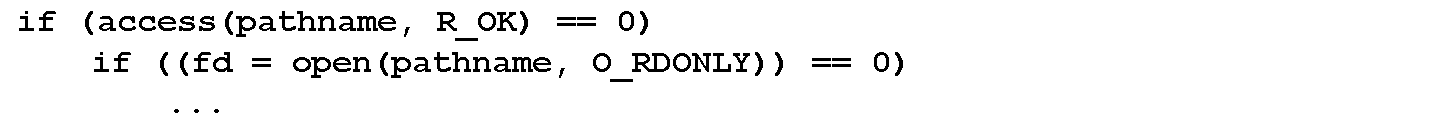
\includegraphics[width=0.47\textwidth]{figures/toctou}
%	\centering
%	\caption{The gap between access() and open() leaves the attack time window for the attacker to make changes in the file system.}
%	\label{fig:toctou}
%\end{figure}
%
%Assume this code piece belongs to a setuid program. It first validates that the ``pathname'' is readable, and if so, open the file for reading. However, the attacker can change the file system between the two system calls to trick the setuid program into opening a file that it should not.



\subsection{Kernel-level TOCTOU Vulnerability}

TOCTOU is a type of vulnerability that involves two references on the same variable or system state. The attacker usually passes the first security check with a benign value and then changes it to a malicious one before the second reference. It is a classic vulnerability, mostly amount file system APIs, which many previous research works have addressed it~\cite{dean2004fixing}~\cite{borisov2005fixing}.


TOCTOU also happens in the operating system kernel. Unlike the classic file system TOCTOU that between APIs, kernel-level TOCTOU happens within individual system calls. When a user program invokes a system call, it usually needs to provide parameters, and it is the kernel's responsibility to verify the legitimacy of the parameters and makes a kernel copy for subsequent use. However, the kernel may fail to accomplish that. Due to the developer's coding style or the unawareness of such vulnerability, the kernel routines do not use the kernel copy of user parameters and fetch the data from userspace again. Even worse, due to various reasons, a kernel module may not fully decouple with the user-mode components, and it directly uses data from userspace.


The double or multiple fetches may lead to severe issues such as local privilege escalation vulnerability. The parameter sent into the kernel is benign initially to pass the security check; then, the attacker alters it to malicious to introduce an error such as a buffer overflow to the kernel. Although the time window between two kernel fetches may be as narrow as several instructions, it is feasible to create the race condition with careful craft, especially on a multi-processor system.


Due to mistakenly repeated operations on user parameters, kernel-level TOCTOU widely exists among operating systems, even in a system such as Linux that use particular gateway functions, \texttt{copy\_to\_user()} and \texttt{copy\_from\_user()}, to get user parameters. ~\autoref{table:cves} lists a portion of recent kernel-level TOCTOU vulnerabilities.


\begin{center}
\begin{table}[ht]
%\singlespacing
%\scalebox{0.8}{
\small
\caption{Recent vulnerabilities categorized as race condition or time-of-check-to-time-of-use in the CVE database.}
\label{table:cves}
\centering
	\begin{tabular}{@{}>{\raggedright\arraybackslash}m{2.35cm}@{}|
			@{}>{\centering\arraybackslash}m{1.35cm}@{}|
			@{}>{\centering\arraybackslash}m{2.35cm}@{}|
			@{}>{\centering\arraybackslash}m{1.25cm}@{} } 
\hline
CVE-ID & Affected System & CVE-ID & Affected System \\ %[0.5ex]
\hline
CVE-2008-2252  & Windows & CVE-2016-5728 & Linux \\
CVE-2013-1280  & Windows & CVE-2016-6130 & Linux \\
CVE-2018-7249  & Windows & CVE-2020-9796 & macOS \\ 
CVE-2020-9839  & macOS   & CVE-2020-9990 & macOS \\
CVE-2016-10439 & Android & CVE-2016-7624 & macOS \\
CVE-2016-10383 & Android & CVE-2017-7115 & iOS \\

CVE-2020-5967  & Nvidia  & CVE-2020-8680 & Intel \\
\hline

\end{tabular}
\end{table}
\end{center}




\begin{figure}[th]
	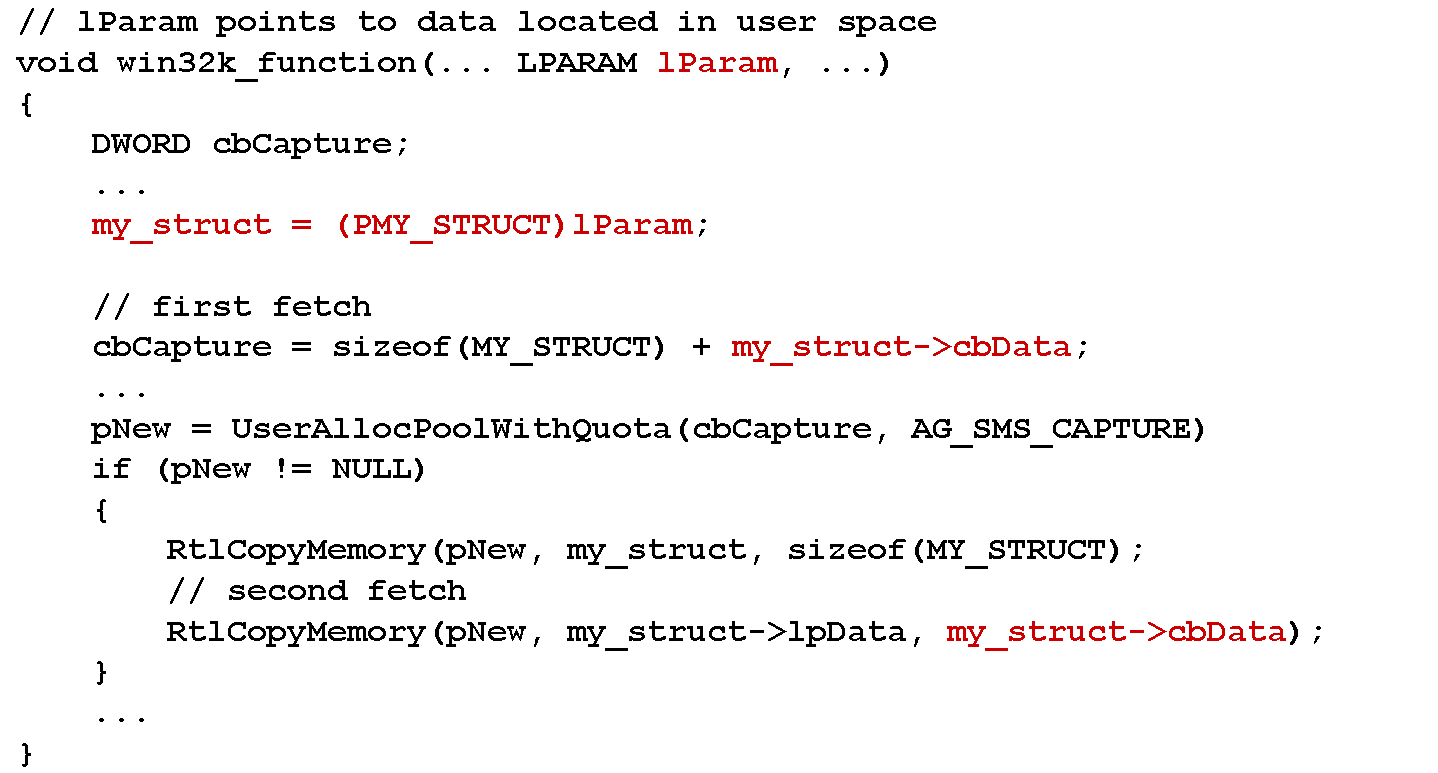
\includegraphics[width=0.47\textwidth]{figures/code08061}
	\centering
	\caption{Pseudocode of the vulnerability fixed in ms08-061. The vulnerable variable is in red. The kernel reads it twice, and it may get a different value for the buffer allocation and the subsequent buffer copying. It is common to see such a coding style. However, it is vulnerable because the two reads cross the privilege boundary.}
	\label{fig:code08061}
\end{figure}




~\autoref{fig:code08061} shows a kernel-level TOCTOU vulnerability pseudo-code from the Windows Win32k module~\cite{jurczyk2013identifying}~\cite{ms08061}. It has been identified and patched in ms08-061. The code belongs to a Win32k system call, and the red part shows the trace of the vulnerable data.  The user program passes \texttt{lParam} to \texttt{win32k\_function()} through upper layer APIs.  Adding \texttt{my\_struct->cbData} to \texttt{cbCapture} is where the kernel first gets this variable and allocates a buffer based on it. Notice, although the variable is called \textit{capture}, the developer forgot to use it subsequently.  Several instructions after, the kernel fetches this variable again when copy data into the new buffer.  An attacker can change the user variable \texttt{my\_struct->cbData} between the two fetches, especially enlarge it. Then it is a kernel buffer overflow.


~\autoref{fig:toctouasm} shows the attack.  To exploit a local privilege escalation vulnerability, the attacker can invoke the vulnerable system call as many times as needed and create another thread to race with the kernel, aiming to enlarge the data during the time window. Thread 1 keeps flipping one higher bit in the variable to make the second fetch's value larger than the first one. It succeeds by chance; otherwise, the attacker can repeat the attack.


\begin{figure}[ht]
  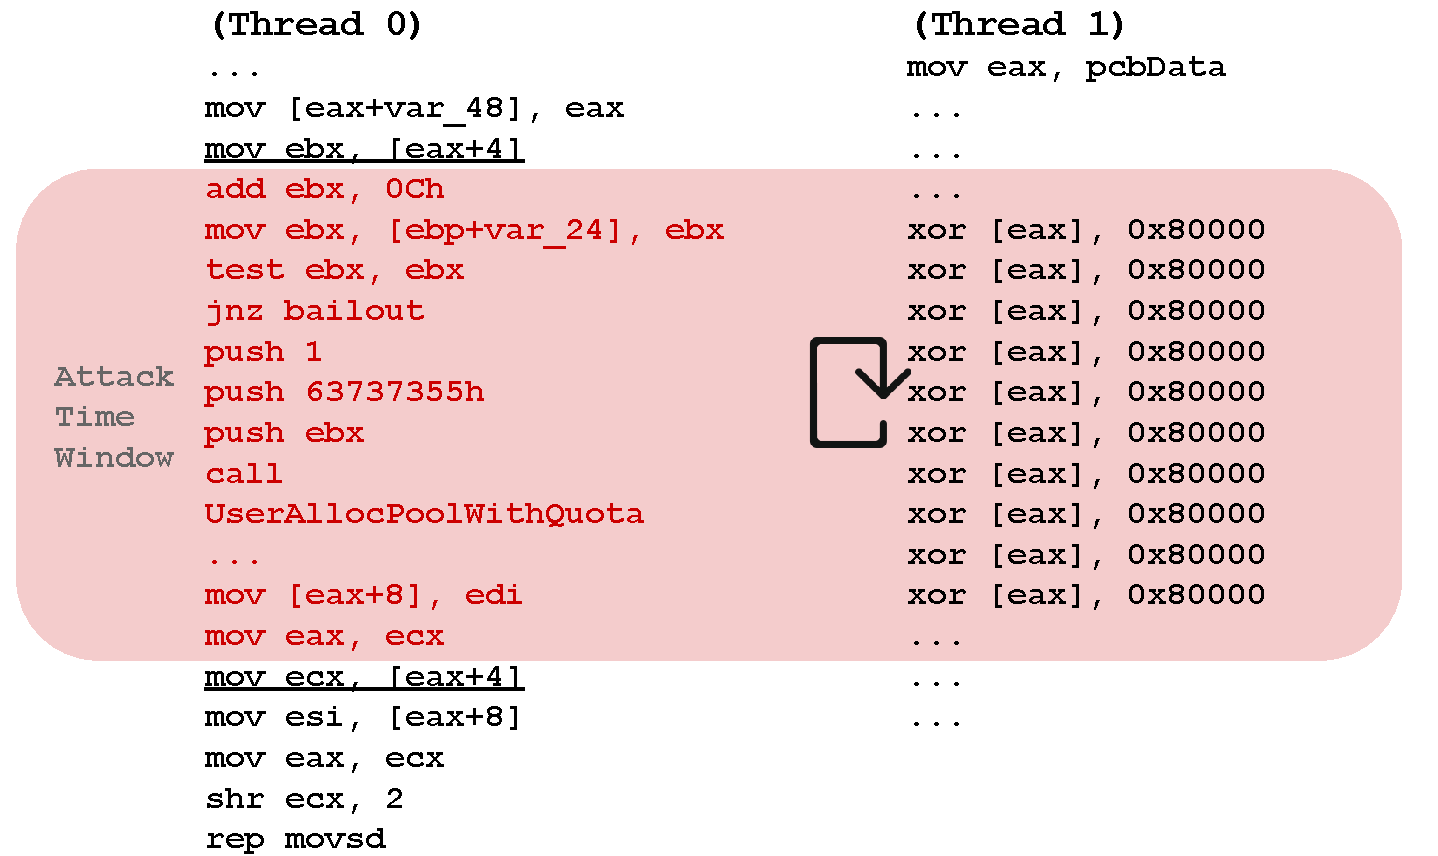
\includegraphics[width=0.47\textwidth]{figures/toctouasm3}
  \centering
  \caption{Thread 0 runs the vulnerable system call in the kernel-mode. The attacker can repeatedly call it to open the attack time window multiple times. Simultaneously, the other user-mode thread created by the attacker tries to flip the user-mode variable in-between the time window. So that the kernel code, two times, get the value differently.}
  \label{fig:toctouasm}
\end{figure}


%Once this step is accomplished, the problem becomes how to exploit it a classic heap buffer overflow. So you can see that kernel TOCTOU itself may not seems to be harmful, but it could lead to something serious. 

\subsection{Supervisor Mode Access Prevention (SMAP)}

Monitoring the kernel's userspace behavior is essential to \name. Due to x86 protected mode characteristics, there is no mechanism available for a broad range of monitoring memory modifications. Techniques such as leveraging hardware watchpoints or transactional memory are fittable for fuzzing such vulnerabilities but not for run-time protection. We discuss these two techniques in more details in~\autoref{sec:ktoctou-experiment} and~\autoref{sec:ktoctou-relatedwork}.

Fortunately, we notice an Intel processor feature so-called Supervisor Mode Access Prevention (SMAP)~\cite{corbet2012supervisorsmap}~\cite{mulnix2016intel} that accurately serves our requirement for monitoring kernel.
SMAP is a feature that prevents the kernel from freely accessing userspace so that such access will raise an exception. It complements Supervisor Mode Execution Prevention (SMEP)~\cite{fischer2011supervisor} that introduced earlier. SMEP can be used to prevent the kernel from unintentionally executing user-mode code. SMAP extends this protection to reads and writes. It makes it harder for a malicious program to deceive the kernel into using code or data from the userspace.

SMAP is enabled when set SMAP (20) bit in CR4 and can be temporarily disabled by setting the AC flag in EFLAGS or through using \texttt{stac} and \texttt{clac} instructions. Temporarily disabling SMAP indicates that the kernel is fully aware of its userspace-access behavior. For example, The Linux kernel supports SMAP since version 3.7. The kernel-to-userspace accesses must go through two gateway functions \texttt{copy\_to\_user()} and \texttt{copy\_from\_user()}, in which SMAP is temporarily disabled.

However, Windows does not support SMAP still. The kernel takes a different approach than gateway functions, that is, \textit{probe} and \textit{capture} user data within each system call. \texttt{ProbeForRead()}~\cite{probeforread} and \texttt{ProbeForWrite()} validates user-mode variables and buffers. This mechanism is effective if done correctly and thoroughly. However, kernel components such as Win32k failed to practice the \textit{probe} and \textit{capture} in a large portion of their code.  The reason is that Win32k is still coupled with user-mode components; it will cost huge engineering effort to change the coding style for the enormous codebase.


\subsection{Intel Virtualization Technology}

Intel Virtual-Machine Extensions (VMX) provides hardware-assistant virtualization, which adds 13 new instructions: VMPTRLD, VMPTRST, VMCLEAR, VMREAD, VMWRITE, VMCALL, VMLAUNCH, VMRESUME, VMXOFF, VMXON, INVEPT, INVVPID, and VMFUNC. VMX supports two modes, namely root and non-root mode, where in root mode runs the hypervisor, and virtual machines or called guest runs in non-root mode. On x86 architecture, the CPU has 4 protection rings, wherethe kernel runs at ring 0, the highest priority ring, and the user programs runs at ring 3, while the other two rings are not used. With VMX, the root model is often viewed as the ring -1. 

VMXON/VMXOFF enters/exits VMX mode. The Virtual Machine Control Structure (VMCS) is the most important data structure, which stores the data and state of one virtual CPU for one virtual machine. Each core in a physical CPU has a VMCS pointer. It points to the physical address of one VMCS. VMPTRLD loads the VMCS pointer from physical memory and makes it active and current. On contrary, VMCLEAR stores VMCS active states back to memory and makes it inactive. Although hypservisor fully aware the physical address of each VMCS but it can not modify them directly. All the operations on VMCS should go through instruction VMREAD and VMWRITE. 

The VMCS contains many data-fields that are related to aspects of a virtual machine. They are organized into six logical groups, namely, Guest-state area, Host-state area, VM-execution control fields, VM-exit control fields, VM-entry control fields, and VM-exit information fields. The last four groups compose VMX controls, which control the virtual machine's behavior such as when to exit to the hypervisor. In VMX's term, VM entry is the transition into the VMX non-root operation while VM exit is the transition from the VMX non-root virtual machine to the VMX root  hypervisor. When VM exit, the processor stores its state into the Guest-state area and loads Host-state area into hardware. In contrast, it loads Guest-state area and stores Host-state area when entering the virtual machine.

\subsection{x86 Architecture}

In this part, we briefly describe background information regarding x86 architecture. These mechanisms are more-or-less use in \name. Topics such as IPI and APIC may fall into this category loosely.

\textbf{\textit{Paging and Virtual Memory.}} On x86 architecture, with the flat or the segmented memory model, linear address space is mapped into the processors' physical memory space either directly or through paging.  Direct mapping is a one-to-one mapping between the linear address and physical address, also known as real-mode. When using the x86 paging mode, the linear address space (often referred to as virtual memory) is divided into pages. For simplicity, we only consider 4KB pages in this paper. The pages of virtual memory are then mapped as needed with physical pages.

Address translation hardware in the processor, often referred to as a Memory Management Unit (MMU), automatically translates virtual addresses to physical addresses with a data structure so-called page table. The translation creates the illusion for every process that it has a large flat virtual memory space (4GB on a 32-bit system).



\textbf{\textit{Page Table.}} The Memory Management Unit (MMU) uses page tables to map physical pages to virtual pages~\cite{intelpaging} so that each process in the system can have a flat virtual memory space. However, to store PTE, the page table's memory usage is unignorable, even on a 32-bit system with a virtual 4GB address. Therefore the page table uses a hierarchy structure to save memory. As shown in~\autoref{fig:pagetable}, the virtual address splits into three parts. The last 12-bit is the byte offset on the page, while the first two 10-bit are the index of the page table base (CR3) and Page Directory (PD). The table is composed of 4KB pages.  The system swaps out long-time unvisited page table pages to save physical memory. 

%As shown in~\autoref{fig:pte}, the least significant bit being zero indicates this page is not present in the physical memory, which brings the following issue. 

When we walk through the page table, it is inevitable to encounter an invalid page-table page, which was not a problem because the system will automatically bring it back by another page fault regarding page absence. However, this becomes a problem since we are already in the context of a SMAP page fault. The swapping process involves the system reading disk, which means more system calls. Due to the reasons mentioned above, system calls inevitably trigger more SMAP exceptions, which form a dead loop. Therefore, to solve this issue brings one of the necessities of developing a hypervisor-based solution to contain SMAP to the process level. 



\begin{figure}[th]
  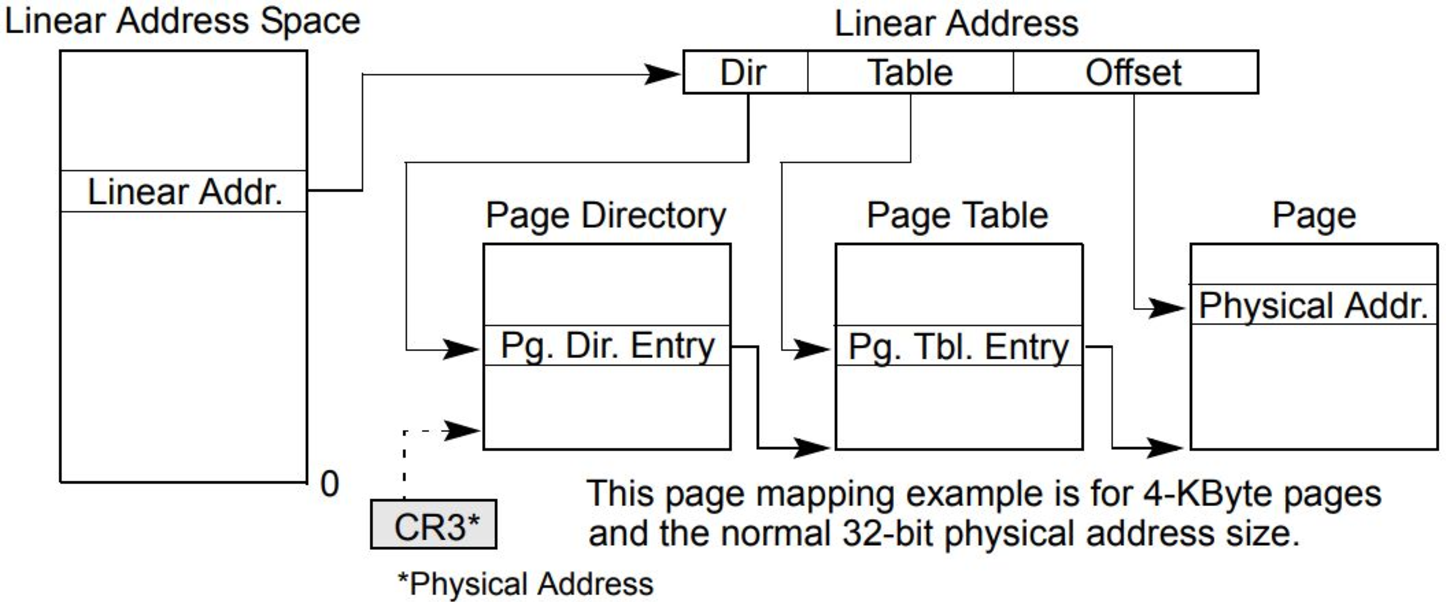
\includegraphics[width=0.47\textwidth]{figures/pagetable}
  \centering
  \caption{Linear-Address Translation to a 4-KBbyte Page using 32-Bit Paging~\cite{guide2011intel}}
  \label{fig:pagetable}
\end{figure}

\textbf{\textit{Translation Lookaside Buffer.}} As mentioned above, page table walking is a lengthy process. A full walk needs to access two pages (PD page and PTE page). If any of the two pages are not present in the memory (PDE or PTE invalid), it further triggers a page fault to bring the absent page back.

A Translation Lookaside Buffer (TLB) is a memory cache used to reduce the time for the processor to access a virtual memory address. It is part of MMU. A TLB has a fixed number of slots that stores the recent translations of virtual memory to physical memory and permission bits.  A TLB may reside between the processor and the processor cache or between the processor cache and the main memory. If valid TLB entry exists, the corresponded PTE is ignored. The system kernel is responsible for the consistency between TLB and page table.



\textbf{\textit{Interrupt Descriptor Table.}} The Interrupt Descriptor Table (IDT) is a data structure used on the x86 architecture to implement an interrupt vector table. The processor uses the IDT to determine the correct response to interrupts and exceptions. IDTR is the register on each processor to store the address of the IDT.

\textbf{\textit{Interrupts and Exceptions.}} The fundamental difference in microarchitecture between interrupt and exception is as follows.  An interrupt is an asynchronous event that is typically triggered by an I/O device. An exception is a synchronous event generated when the processor detects one or more predefined conditions while executing an instruction. However, one thing in common is that their handlers are all in the IDT, which makes them easy to confuse.

Furthermore, exceptions are classified as \textbf{faults}, \textbf{traps}, and \textbf{aborts} depending on the way they are reported and whether the instruction that caused the exception can be restarted without loss of program or task continuity. Aborts are not recoverable. They are used to report severe errors, such as hardware errors and inconsistent or illegal values in system tables. Faults and traps are recoverable, and the main difference between them is that when recovers from faults, the return address is the faulting instruction. On the other side, the trap's return address points to the instruction to be executed after the trapping instruction. In our case, the SMAP exception is a fault and handled through the page fault handler.

The IDT has 256 entries. Entry 0-31 are for exceptions except the entry 2 is for Non-Maskable external Interrupt (NMI). The rest are for external interrupt from INTR pin or INT n instruction. However, INT n also known as a software interrupt. It is essentially an exception with "interrupt" in its name, and its vector located with other external hardware interrupt vectors. Fun.



\textbf{\textit{Trap Frame.}} It is the data structure pushed to the stack by the processor. It contains registers of the current thread when an interrupt or exception occurs. Each trap frame stores only a subset of the registers depending on scenarios, namely, the SS:ESP is pushed base on if there is a change in Current Privilege Level (CPL) of the CS register.  In the context of a page fault, ErrorCode, CS:EIP, EFLAGS, and SS:ESP are pushed into the kernel stack.



\textbf{\textit{Gate.}} Code modules in lower privilege segments can only access modules operating at higher privilege segments through a tightly controlled and protected interface called a \textbf{gate}.  There are four types of gate, namely, \textbf{task gate}, \textbf{trap gate}, \textbf{interrupt gate}, and \textbf{call gate}. Fully describe and distinguish them is out of the paper's scope. The project only involves the interrupt gate.

The vectors in the IDT go through either the interrupt gate or trap gate. The difference between them is as follows. If the interrupt or exception handler is called through an interrupt gate, the processor clears the interrupt enable flag (IF) in the EFLAGS register to prevent subsequent interrupts from interfering with the execution of the handler.  When the processor invokes a handler through a trap gate, it does not change the IF flag. Having EFLAGS.IF set is a requirement to control stack depth, which also involves what type of interrupt controller installed in the system. We observed that the processor invokes the page fault handler through an interrupt gate. We think the reason for that is as follows. The processor loads the CR2 register with the 32-bit virtual address that generated the exception. Another page fault can potentially occur during the execution of the page fault handler. Hence the page fault handler should save the contents of the CR2 before a second page fault can occur because the processor update CR2 whenever a page fault is detected.

\textbf{\textit{CS Segment and Current Privilege Level}} CS segment register cannot be set directly through instruction mov, unlike other segment registers,  but only through a trap or interrupt gate. The system's current privilege level depends on the Current Privilege Level (CPL) field in the CS segment, which is maintained by the processor. This 2-bit CPL field in the code segment register is always equal to the processor's current privilege level. When getting the CS image from the trap frame of a page fault context, it provides us the ground truth of what privilege of the code when the SMAP exception happens, so that we do not make the decision based on the apparent value of EIP. To fully explain the privilege transition mechanism is out of the paper's scope.

\textbf{\textit{Inter-processor Interrupt.}}  It is an interrupt controller mechanism to interrupt another processor or group of processors on the system bus. They are used for software self-interrupts, interrupt forwarding, or preemptive scheduling. In \name, we use IPI to flush TLB cache on all the processors.

\textbf{\textit{Local APIC.}} Intel's Advanced Programmable Interrupt Controller (APIC) is a family of interrupt controllers. It is more advanced than Intel's 8259 Programmable Interrupt Controller (PIC). Nowadays, SMP systems with multiple processors utilize APIC. The APIC is a split architecture design, with a local APIC usually integrated into the processor and an optional I/O APIC on a system bus. The local APIC performs two primary functions for the processor:
It receives interrupts from the processor's interrupt pins, internal sources, and an external I/O APIC. It sends these to the processor core for handling.
It sends and receives IPI messages to and from other logical processors on the system bus in multiple-processor systems.
The external I/O APIC is part of Intel's system chipset. It is responsible for receiving interrupts generated by system hardware and I/O devices and forwarding them to the local APIC as interrupt messages. A processor can generate IPIs by programming the interrupt command register (ICR) in its local APIC. Writing to the ICR generates an IPI message on the system bus or the APIC bus. When the target processor receives an IPI message, its local APIC handles the message automatically using information included in the message such as vector number and trigger mode. The IPI mechanism sends interrupts for a specific vector number, and special-purpose interrupts to processors on the system bus. Local APIC registers are memory-mapped to a 4-KByte region of the processor's physical address space with an initial starting address of EFF00000H. The software interacts with the local APIC by reading and writing its registers. It also can change the initial mapping to a different 4-KByte region for all the local APICs. The presence of a local APIC can be detected using the CPUID instruction. Execute CPUID with source operand of 1 in the EAX register, then bit 9 of returned feature flags in EDX register indicate a local APIC.


\begin{figure}[th]
  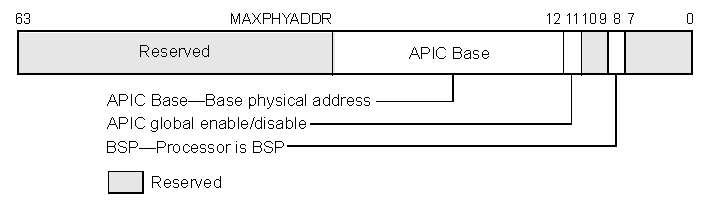
\includegraphics[width=0.47\textwidth]{figures/ia32apicbase}
  \centering
  \caption{\texttt{IA32\_APIC\_BASE MSR}}
  \label{fig:ia32apicbase}
\end{figure}

There is only one MSR associated with local APIC, \texttt{IA32\_APIC\_BASE}. As shown in~\autoref{fig:ia32apicbase}, the BSP flag indicates if the processor is the bootstrap processor (BSP); ``APIC global enable/disable'' enables/disables the APIC; APIC base specifies the base address of the APIC registers. This 24-bit value needs to be extended by 12 bits at the low end to form the base address. As formerly mentioned, this value by default is 0xFEE00000.

The primary local APIC facility for issuing IPIs is the interrupt command register (ICR), as shown in~\autoref{fig:icr}. It is a 64-bit local APIC register that allows the operating system to specify and send IPIs to processors in the system.


\begin{figure}[th]
  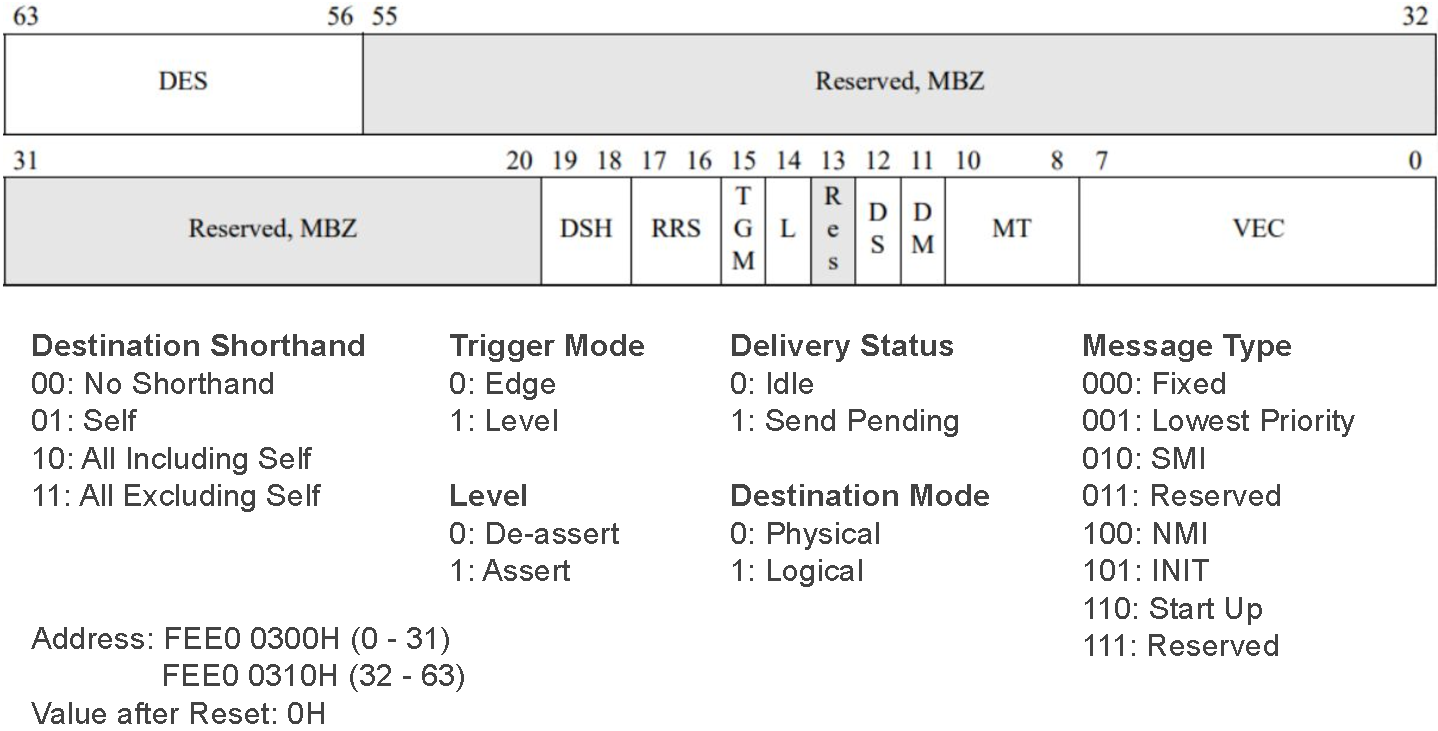
\includegraphics[width=0.47\textwidth]{figures/icr2}
  \centering
  \caption{Interrupt Command Register (ICR). Notice, Intel and AMD has slightly different definitions.~\cite{intelapic}~\cite{amdapic}}
  \label{fig:icr}
\end{figure}

